\section{账户管理}
\subsection{Accounts9账号登陆}
系统支持用户使用Accounts9账号进行登陆。Accounts9使用OAuth2.0协议,其流程如下图所示:
\begin{center}
    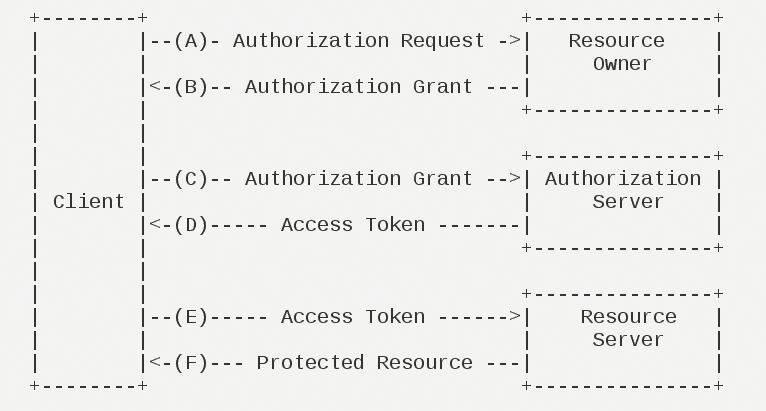
\includegraphics[width=14cm]{image/account/oauth.png}
    \fcaption{OAuth 2.0运行流程}
\end{center}
用户登出时,系统会将其重定向到Accounts9的页面,提示用户将Accounts9下线。

\subsection{访问权限控制}
一期工程中虽然区分了学生和管理员两类用户,但其区别仅仅体现在登陆后进入到不同的界面,对系统之后的运行过程中的用户访问权限并没有进行检查,例如学生可以通过修改URL地址栏而进入到管理员端。二期工程修复了这一问题,对于学生和管理员,通过核查authority域阻止权限非法的操作。此外,在涉及到与项目有关的操作时,也会在数据库中检查该项目id是否属于当前用户。

\subsection{同一账户多次登陆}
对于同一个浏览器,允许相同的账户多次登陆,均可以正常操作,且由于浏览器的本地缓存,再次访问实验平台时会跳过登陆界面,直接进入主页面。当用户登出时,此次会话的全部状态信息会被清空,此时若当前浏览器还存在该账户的其他登陆,则其下一步操作会跳转到登陆界面。

对于不同的浏览器,新的登陆会使前一次的登陆状态无效。即若用户用另一个浏览器再次登陆实验平台时,在前一个浏览器中的任何操作均会使会话的状态信息清空,从而跳转到登陆界面。这一机制是通过Accounts9返回的access token实现的,系统会用新的access token覆盖掉数据库中原有的该账户的access token,这样第一次登陆时获得的access token与服务器当前存储的access token就会失配。